\documentclass[conference]{IEEEtran}
\usepackage[T1]{fontenc}
\usepackage{amsmath,amssymb}
\usepackage{graphicx}
\usepackage{xcolor}
\usepackage{tikz}
\usetikzlibrary{shapes.geometric,arrows.meta,positioning,fit}
\usepackage{booktabs}
\usepackage{multirow}
\usepackage{url}

\newcommand{\TBD}{\textcolor{red}{\textbf{[TBD]}}}
\newcommand{\code}[1]{\texttt{#1}}

\begin{document}

\title{Vehicle Classification, Multi-Object Tracking and Counting, and
Speed Estimation on a Grid-Based Motion-Detection Baseline: Sequential
and Parallel Implementations with a Fair-Comparison Evaluation}

\author{
\IEEEauthorblockN{Jay Suriya R}
\IEEEauthorblockA{Department of Computer Science and Engineering\\
Indian Institute of Information Technology Sri City\\
Sri City, India\\
jaysuriya.r24@iiits.in}
\and
\IEEEauthorblockN{Manipriya Sankaranarayanan}
\IEEEauthorblockA{Department of Computer Science and Engineering\\
Indian Institute of Information Technology Sri City\\
Sri City, India\\
manipriya.s@iiits.in}
}

\maketitle

\begin{abstract}
A prior published system \cite{baseline} performs grid-based vehicle
motion detection: a region of interest (ROI) is discretized into a
grid, histogram-equalized frame differencing marks each cell as
motion/no-motion, and a preliminary dual-ROI implementation dispatches
this per-cell work across a freshly created thread pool every frame.
That baseline stops at a binary occupancy grid -- it does not classify
vehicles, track individuals across frames, count crossings, estimate
speed, or evaluate against ground truth. This paper documents that
work, built entirely on top of the baseline's motion-detection front
end: rule-based vehicle classification from per-cluster grid geometry,
multi-object tracking with temporally smoothed labels and
duplicate-aware line-crossing counting, displacement-gated speed
estimation, and adaptively thresholded traffic-density estimation --
implemented and evaluated in \emph{both} a sequential form and a
substantially redesigned parallel form. The baseline's naive
per-frame thread-pool recreation cannot hold state across frames, which
per-vehicle tracking, classification smoothing, and speed estimation all
require; this paper's parallel implementation instead encapsulates all
per-lane tracking state in a \code{LaneTracker} class driven by two
persistent \code{ThreadPoolExecutor} pools, with an explicit compute/draw
separation that keeps the two lanes race-free on the shared frame
buffer. We evaluate both implementations against UA-DETRAC ground truth
and report a benchmarking protocol that corrects for a workload confound
between them (one versus two ROIs per frame) via a workload-normalized
throughput metric. A cross-implementation validation check -- comparing
per-video DETRAC confusion matrices between the sequential
implementation and the parallel implementation's first lane, which
should be identical given supposedly-identical tracking/classification
logic on the same ROI -- surfaced two real preprocessing divergences in
the underlying frame-differencing step (a missing pre-differencing
Gaussian blur, introduced when this work extended the baseline's
sequential preprocessing but not correspondingly ported to the parallel
side; and a histogram-equalization method that silently discarded color
information, present unchanged in the published baseline's parallel
code since before this work began) that had been masking the
implementations' true relative performance. After fixing both, all 12
benchmark videos (drawn from UA-DETRAC's Cloudy/Night/Rainy/Sunny
categories across light/medium/heavy traffic-density tiers) produce
bit-identical classification results between implementations. On this
corrected basis, the workload-normalized speedup of the parallel
implementation is a modest $1.261\times \pm 0.084$ ($n{=}12$) -- not the
$\sim$3.3$\times$ an uncorrected wall-clock measurement had initially
suggested before an unrelated timing-instrumentation artifact (an
unthrottled \code{cv2.waitKey} poll and an asymmetric per-frame disk
write) was also found and fixed. Per-stage \code{cProfile} analysis
shows this modest speedup is well predicted by an Amdahl's-law estimate
restricted to the fraction of work actually dispatched to the thread
pool ($p{\approx}0.39$, predicting $1.24\times$ at the pool's effective
concurrency width of 2) rather than by the broader fraction of the
pipeline that merely happens to call native code ($p{\approx}0.67$,
predicting $3.0\times$), and that speedup degrades further under
heavier traffic density as the unparallelized, pure-Python
tracking-bookkeeping stage this work adds grows with vehicle count. We
report full accuracy and timing breakdowns by weather category and
density tier, and document both the benchmarking artifacts and the
algorithmic divergences found in the course of this work as evidence
for a general point: an ``identical algorithm, parallelized'' claim
between independently maintained code paths is an empirical claim that
drifts silently and must be re-verified, not assumed from documentation.
\end{abstract}

\begin{IEEEkeywords}
vehicle classification, multi-object tracking, vehicle counting, speed
estimation, traffic density estimation, parallel computing, thread
pool, Python GIL, UA-DETRAC
\end{IEEEkeywords}

\section{Introduction}
\label{sec:intro}

Automated traffic monitoring increasingly relies on video analytics to
count vehicles, estimate speed, and classify vehicle type without
dedicated inductive-loop or radar hardware. The dominant approach in
recent literature is a learned object detector (e.g., a convolutional or
transformer-based network) combined with a tracking-by-detection
algorithm. These systems are accurate but computationally expensive,
which is a real constraint for edge deployments -- roadside units,
low-power embedded cameras, or software running alongside other
processes on shared hardware -- where a GPU or a large CPU budget is not
guaranteed to be available for every camera stream.

\subsection{Relationship to Prior Published Work}
\label{sec:priorwork}
A previously published system \cite{baseline} addresses the motion-detection
front end of this problem without a learned detector: each region of
interest (ROI) is discretized into a grid; consecutive frames are
histogram-equalized and differenced; and each grid cell is independently
marked motion/no-motion via per-cell blur-threshold-dilate-contour
detection. That system also includes a preliminary dual-ROI
implementation that dispatches this per-cell work across a thread pool.
Section~\ref{sec:overview} describes this baseline in the detail needed
to establish the notation used throughout the rest of the paper, and
Table~\ref{tab:baseline-vs-contribution} summarizes the boundary
precisely. \textbf{The baseline stops at a binary per-cell occupancy
grid.} It performs no vehicle classification, no per-vehicle tracking
or identity assignment, no line-crossing counting, no speed estimation,
no adaptively thresholded density estimation, and no evaluation against
ground truth; its preliminary parallel implementation recreates a thread
pool every frame and holds no state across frames.

This paper documents everything built on top of that occupancy grid:
rule-based vehicle classification from the geometry of clustered hot
cells; multi-object tracking with temporally smoothed labels,
duplicate-track suppression, and duplicate-crossing-aware vehicle
counting; displacement-gated speed estimation; and adaptively
thresholded traffic-density estimation combining spatial occupancy with
recent flow -- implemented and evaluated in \emph{both} a sequential
form and a parallel form. Critically, per-vehicle tracking,
label-smoothing, and speed estimation all require state that persists
across frames per lane, which the baseline's per-frame thread-pool
recreation cannot hold; supporting these features in a parallel
implementation therefore required a substantially redesigned
concurrency architecture, described in Section~\ref{sec:parallel}, not
a direct reuse of the baseline's preliminary threading.

We implement and document two versions of the resulting system:

\begin{itemize}
\item \textbf{Sequential (\code{seq.py})}: a single-lane, procedural
implementation using module-level global state, instrumented with
per-frame timing, memory sampling, and \code{cProfile}-based
function-level profiling.
\item \textbf{Parallel (\code{rparallel\_he3.py})}: a dual-lane
implementation that encapsulates all per-lane tracking state in a
\code{LaneTracker} class and dispatches (i) the $O(\text{rows}\times
\text{cols})$ per-cell contour computations and (ii) the two lanes'
grid-detection and tracking-state updates across two persistent
\code{ThreadPoolExecutor} pools.
\end{itemize}

The two implementations are intended to be algorithmically identical in
every stage except lane count, which would let us isolate the effect of
the concurrency architecture alone -- but, as Section~\ref{sec:discussion}
reports, that intended equivalence was not automatic and had to be
verified and repaired. Comparing them also introduces a workload
confound (one ROI vs.\ two ROIs per frame) that a naive wall-clock
comparison would silently absorb into an inflated or deflated
``speedup'' number. Section~\ref{sec:experiments} makes this confound
explicit and defines a workload-normalized throughput metric so that
reported speedup numbers reflect the concurrency architecture and not
simply a doubled workload.

\begin{table}[t]
\centering
\caption{What is prior published work \cite{baseline} vs.\ this
paper's contribution.}
\label{tab:baseline-vs-contribution}
\footnotesize
\begin{tabular}{p{3.9cm}p{3.6cm}}
\toprule
\textbf{Prior work \cite{baseline} (baseline)} & \textbf{This paper} \\
\midrule
ROI grid discretization &
Spatial clustering of hot cells into vehicle-sized objects
(Section~\ref{sec:cluster}) \\
Per-cell motion detection (blur/threshold/dilate/contour) &
Retuned per-cell detection parameters to support geometric classification
(Section~\ref{sec:motion}) \\
Histogram-equalized frame differencing &
-- (reused; two latent bugs in it found and fixed, Section~\ref{sec:discussion}) \\
-- &
Rule-based vehicle classification (Section~\ref{sec:classify}) \\
-- &
Multi-object tracking, duplicate suppression, line-crossing counting
(Section~\ref{sec:tracking}) \\
-- &
Displacement-gated speed estimation (Section~\ref{sec:tracking}E) \\
Raw occupancy fraction (printed, not thresholded) &
Adaptive percentile-based density thresholding with flow blending
(Section~\ref{sec:density}) \\
Preliminary per-frame thread-pool recreation, stateless &
Persistent, stateful two-pool architecture with per-lane
\code{LaneTracker} encapsulation (Section~\ref{sec:parallel}) \\
-- &
DETRAC ground-truth evaluation methodology (Section~\ref{sec:eval}) \\
-- &
Fair-comparison benchmarking protocol and cross-implementation
validation (Sections~\ref{sec:experiments}--\ref{sec:discussion}) \\
\bottomrule
\end{tabular}
\end{table}

This work builds on that baseline through five contributions:
1) a rule-based vehicle classification, multi-object tracking and
counting, and speed-estimation layer, together with every hand-tuned
constant that governs its behavior (Table~\ref{tab:params}),
implemented identically in both a sequential and a parallel execution
model; 2) an adaptively thresholded traffic-density estimator that
extends the baseline's raw per-frame occupancy fraction with
percentile-based recalibration and flow blending
(Section~\ref{sec:density}); 3) a substantially redesigned concurrency
architecture -- two persistent thread pools and per-lane
\code{LaneTracker} state encapsulation -- required because the new
tracking/classification/speed layer needs cross-frame state per lane
that the baseline's preliminary, stateless, per-frame thread-pool
recreation cannot provide (Section~\ref{sec:parallel}), with an
explicit argument for \emph{why} and \emph{where} GIL-releasing native
calls make thread-based parallelism viable for this added workload,
and where they do not; 4) a DETRAC-grounded evaluation methodology
covering both grid-level and vehicle-level (ID-based) accuracy,
applied identically to both implementations (Section~\ref{sec:eval}) --
the baseline has no evaluation methodology to extend; and 5) a
benchmarking protocol and an accompanying analysis script
(\code{analyze\_results.py}) that reports a workload-normalized speedup
figure correcting for the one-lane-vs-two-lane confound between the
two implementations (Section~\ref{sec:experiments}), together with a
cross-implementation validation methodology that found and fixed two
real accuracy-affecting divergences in the reused preprocessing step
before trusting any comparison built on top of it
(Section~\ref{sec:discussion}).

\section{Related Work}
\label{sec:related}

The grid-based motion-detection front end this paper builds on --
ROI discretization, histogram-equalized frame differencing, and
per-cell blur-threshold-dilate-contour occupancy detection, together
with a preliminary dual-ROI threaded implementation -- is prior
published work \cite{baseline}. This paper does not re-claim that
front end; Section~\ref{sec:overview} and Table~\ref{tab:baseline-vs-contribution}
describe it only to the extent needed to establish notation, and every
subsequent section is explicit about which parts are reused unchanged,
which are retuned, and which are new.

Frame differencing and background subtraction remain widely used for
motion detection in traffic video because of their low computational
cost relative to learned detectors. Cheung and Kamath compare simple
frame-differencing and adaptive median filtering against more elaborate
probabilistic background models for urban traffic video and find that
the simpler techniques remain competitive at a fraction of the
computational cost \cite{cheung2004}, which is consistent with the
motivation for the baseline's frame-differencing-plus-grid design.
Contour extraction from the resulting binary motion masks -- used
throughout the baseline and this paper via OpenCV's
\code{cv2.findContours} -- implements the border-following algorithm of
Suzuki and Abe \cite{suzuki1985}.

A separate, contemporaneous extension of the same baseline
\cite{muthuraja2026} pursues a complementary direction: scene-adaptive
preprocessing (per-frame illumination classification, CLAHE, and a Dark
Channel Prior degradation indicator) and perspective-aware centroid
non-maximum suppression, evaluated on 60 UA-DETRAC sequences with a
Hungarian-matched protocol and reporting 71.03\% micro-averaged F1. That
work explicitly notes the baseline ``reports execution time and memory
consumption but does not provide detection-accuracy metrics,'' and adds
an accuracy evaluation without addressing parallelization. The present
paper is complementary in the other direction: it adds no scene-adaptive
preprocessing, but adds vehicle classification, multi-object tracking
and counting, speed estimation, and -- unlike either prior work -- a
verified-equivalent sequential/parallel comparison methodology.

Evaluation is performed against the UA-DETRAC benchmark, a large-scale
traffic video dataset with per-frame, per-vehicle bounding-box and
type annotations designed for joint detection-and-tracking evaluation
\cite{wen2020}. We reuse its vehicle-type taxonomy (car, van, bus, and an
``others''/unknown category) as the target label space for the
classification stage.

On the systems side, CPython's Global Interpreter Lock (GIL) serializes
execution of Python bytecode across threads within a single process
\cite{pythongil}; \code{concurrent.futures.ThreadPoolExecutor}
\cite{pythonfutures} is nonetheless an effective concurrency primitive
for workloads dominated by calls into C/C++ extensions -- such as
OpenCV's \code{GaussianBlur}, \code{threshold}, \code{dilate}, and
\code{findContours} -- because those calls release the GIL for their
duration. The theoretical ceiling on any such speedup, as a function of
the parallelizable fraction $p$ of the workload and the number of
workers $N$, is given by Amdahl's law \cite{amdahl1967}:
\begin{equation}
S(N) = \frac{1}{(1-p) + p/N}.
\label{eq:amdahl}
\end{equation}
Section~\ref{sec:results} uses Eq.~\eqref{eq:amdahl} as a reference
ceiling against which the measured speedup is compared.

\section{Proposed Methodology}
\label{sec:methodology}

\subsection{System Overview}
\label{sec:overview}

\textbf{What is baseline, briefly.} The prior published system
\cite{baseline} discretizes each ROI into a grid, histogram-equalizes
and differences consecutive frames, and marks each cell
motion/no-motion via per-cell blur-threshold-dilate-contour detection,
producing a binary occupancy grid per frame. Its preliminary parallel
implementation dispatches this per-cell work across a thread pool
recreated every frame and holds no state across frames. Nothing past
this point -- clustering, classification, tracking, counting, speed,
adaptive density, or evaluation -- exists in the baseline.

\textbf{What this paper adds.} Both implementations documented here
share the pipeline shown in Fig.~\ref{fig:pipeline}: two consecutive
frames are read from the video; the ROI(s) are histogram-equalized and
blurred (baseline preprocessing, Section~\ref{sec:motion}, reused with
retuned per-cell parameters and two latent bugs found and fixed --
Section~\ref{sec:discussion}); a channel-selected absolute difference is
computed and each grid cell is marked motion/no-motion (baseline); from
this point on, everything is this paper's contribution: ``hot'' cells
are flood-fill clustered into candidate vehicle objects
(Section~\ref{sec:cluster}); each cluster is classified by its grid
footprint (Section~\ref{sec:classify}); clusters are associated to
existing tracks or spawn new ones, accumulate temporally smoothed
labels, crossing counts, and speed estimates (Section~\ref{sec:tracking});
and the frame is annotated and written to disk alongside an adaptively
thresholded traffic-density estimate (Section~\ref{sec:density}). The
sequential implementation applies this to a single ROI (\code{roi1});
the parallel implementation applies it to two ROIs (\code{roi1},
\code{roi2}) representing two independent lanes, via the redesigned
concurrency architecture of Section~\ref{sec:parallel}.\footnote{This
equivalence was not automatic: a benchmarking cross-check
(Section~\ref{sec:discussion}) found \emph{two} preprocessing
divergences between the implementations, found and fixed sequentially
because the first fix alone did not resolve the accuracy mismatch. (1)
The frame-level $7\times7$ Gaussian blur applied before differencing in
\code{seq.py}'s \code{process\_hsv}/\code{process\_grayscale} was added
when this work extended the baseline's sequential preprocessing, but
was not correspondingly ported to the parallel implementation's
equivalent functions -- it is absent from the baseline itself, on
either side. (2) \code{seq.py}'s histogram equalization equalizes only
the V channel in HSV space (\code{he\_choice='V'}), preserving hue and
saturation, and this branching logic is present unchanged from the
baseline; the parallel implementation's equivalent function, also
unchanged from the baseline, ignored \code{channel\_choice} entirely and
always collapsed the ROI to grayscale before equalizing -- a materially
different preprocessing step that predates this work and went unnoticed
because the baseline's occupancy-only output is far less sensitive to
it than the classification stage added here. Both have been added to
the parallel implementation to match \code{seq.py} exactly;
\code{seq.py} itself was not modified. All results in this paper reflect
the corrected, verified-equivalent version.}

\begin{figure*}[t]
\centering
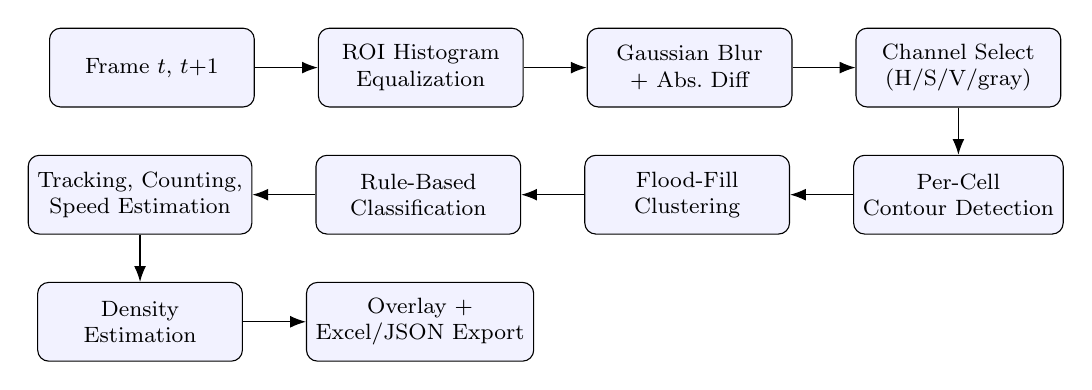
\begin{tikzpicture}[
  node distance=6mm and 8mm,
  box/.style={draw, rounded corners, align=center, minimum height=1.0cm,
              minimum width=2.6cm, font=\footnotesize, fill=blue!5},
  arr/.style={-{Latex[length=2mm]}}
]
\node[box] (frames) {Frame $t$, $t{+}1$};
\node[box, right=of frames] (he) {ROI Histogram\\Equalization};
\node[box, right=of he] (diff) {Gaussian Blur\\+ Abs.\ Diff};
\node[box, right=of diff] (chan) {Channel Select\\(H/S/V/gray)};
\node[box, below=of chan] (cell) {Per-Cell\\Contour Detection};
\node[box, left=of cell] (cluster) {Flood-Fill\\Clustering};
\node[box, left=of cluster] (classify) {Rule-Based\\Classification};
\node[box, left=of classify] (track) {Tracking, Counting,\\Speed Estimation};
\node[box, below=of track] (density) {Density\\Estimation};
\node[box, right=of density] (overlay) {Overlay +\\Excel/JSON Export};

\draw[arr] (frames) -- (he);
\draw[arr] (he) -- (diff);
\draw[arr] (diff) -- (chan);
\draw[arr] (chan) -- (cell);
\draw[arr] (cell) -- (cluster);
\draw[arr] (cluster) -- (classify);
\draw[arr] (classify) -- (track);
\draw[arr] (track) -- (density);
\draw[arr] (density) -- (overlay);
\end{tikzpicture}
\caption{Per-ROI processing pipeline shared by both implementations.
The sequential implementation runs one instance of this pipeline per
frame (ROI~1 only); the parallel implementation runs two instances per
frame (ROI~1 and ROI~2), dispatched as described in
Section~\ref{sec:parallel} and Fig.~\ref{fig:threadpools}.}
\label{fig:pipeline}
\end{figure*}

\subsection{Grid-Based Motion Detection}
\label{sec:motion}

This section's motion-detection front end is prior published work
\cite{baseline}, reused here as the input to the classification and
tracking layers of Sections~\ref{sec:cluster}--\ref{sec:tracking}. It is
described only to the depth needed to fix notation and to document two
adaptations made in the course of this work: the per-cell detection
thresholds were retuned (Section~\ref{sec:motion}C) because the
classification stage added here depends on precise contour geometry in
a way the baseline's simple occupancy check did not, and two latent
preprocessing bugs in the reused code were found and fixed
(Section~\ref{sec:discussion}).

\subsubsection{Contrast Normalization}
Before differencing, the pipeline applies histogram equalization
restricted to the ROI. Two modes are supported: full grayscale
equalization of the ROI (\code{cv2.equalizeHist} applied after a
grayscale conversion), or equalization of a single HSV channel (H, S,
or V) with the other two channels left unmodified before converting
back to BGR. This is applied independently to both input frames prior
to differencing, so that the differencing step operates on
contrast-normalized ROIs rather than raw pixel intensities, which
reduces sensitivity to slow lighting drift across the sequence.

\subsubsection{Frame Differencing and Channel Selection}
Both equalized frames are Gaussian-blurred ($7\times7$ kernel) and
absolute-differenced. The result is converted to HSV, and a
configurable subset of channels is split out (H, S, V, or any
combination, or plain grayscale via a separate \code{gray} code path).
This is a user-facing configuration knob (\code{color\_channel} in
\code{user\_input\_data.json}) that trades sensitivity to
illumination-only motion (grayscale/V) against sensitivity to
hue/saturation-varying motion (H/S), and directly determines how many
independent per-cell contour computations are required (one per
selected channel).

\subsubsection{Per-Cell Contour Detection}
Each grid cell of each selected channel image is independently
Gaussian-blurred ($5\times5$), thresholded at a fixed intensity of 60,
and dilated with a rectangular structuring element sized to the cell
itself (\code{grid\_width} $\times$ \code{grid\_height}/2, 5 iterations)
to bridge small gaps in a vehicle's motion silhouette before contour
extraction via \code{cv2.findContours} (Suzuki--Abe border following
\cite{suzuki1985}). A contour is accepted only if its area exceeds 100
px$^2$. A cell is marked ``hot'' (binary result matrix entry $=1$)
\emph{only if every selected channel independently reports at least one
valid contour} -- an AND-across-channels rule intended to suppress
motion detected in only one channel (e.g., a shadow that perturbs V but
not H or S).

Relative to the baseline \cite{baseline}, this work retuned four of
these parameters -- the threshold intensity (20 $\to$ 60), the dilation
kernel (a fixed, cell-independent kernel with 3 iterations $\to$ a
cell-sized kernel with 5 iterations), the contour retrieval mode
(\code{RETR\_TREE} $\to$ \code{RETR\_EXTERNAL}), and the blur's sigma
(0 $\to$ 1) -- because Section~\ref{sec:classify}'s classifier depends
on a cluster's precise \code{col\_span}/\code{row\_span}, which is far
more sensitive to over- or under-dilated, nested, or noisy contours
than the baseline's simple presence/absence occupancy check ever was.
The minimum contour area (100 px$^2$) is unchanged from the baseline.

\begin{table}[t]
\centering
\caption{Key pipeline parameters (identical in both implementations
unless noted).}
\label{tab:params}
\footnotesize
\begin{tabular}{p{3.6cm}p{3.9cm}}
\toprule
\textbf{Parameter} & \textbf{Value} \\
\midrule
ROI~1 (x, y, w, h) & (47, 202, 441, 141) \\
ROI~2 (x, y, w, h), parallel only & (500, 202, 441, 141) \\
Grid dimensions (rows $\times$ cols) & configurable, \code{user\_input\_data.json} \\
Cell blur / threshold & $5\times5$ Gaussian, $T{=}60$ \\
Cell dilation & (cell\_w, cell\_h/2) kernel, 5 iters \\
Min.\ contour area (cell) & 100 px$^2$ \\
Frame-diff blur & $7\times7$ Gaussian \\
Track match radius & ROI height / 2 \\
Duplicate-track IoU threshold & 0.40 \\
Crossing cooldown & 30 frames, 60 px \\
Label EWA $\alpha$ & 0.15 \\
Min.\ frames before label scored & 5 \\
Min.\ speed sample displacement & 3 $\times$ grid-cell height \\
Speed smoothing window & last 15 samples \\
Density blend weights & 0.7 (smoothed) / 0.3 (flow) \\
Density base thresholds & 0.25 (Low/Med), 0.55 (Med/High) \\
Density threshold adaptation & $\pm$0.10, active after $>$50 samples \\
Assumed max flow & 8 vehicles/s \\
\code{\_CELL\_POOL} size (parallel) & $\min(32, 4\times\text{cpu\_count})$ \\
\code{\_LANE\_POOL} size (parallel) & 2 \\
\bottomrule
\end{tabular}
\end{table}

\subsection{Spatial Clustering and Object Formation}
\label{sec:cluster}

The baseline \cite{baseline} stops at the per-cell binary occupancy grid
of Section~\ref{sec:motion}; everything from this section onward is
this paper's contribution, starting with converting that occupancy grid
into discrete, per-vehicle candidate objects.

Hot cells are grouped into candidate vehicle objects by 4-connected
flood fill (\code{group\_cells}): starting from any unvisited hot cell,
a depth-first search over its row/column neighbors collects a maximal
connected component of hot cells, repeated until every hot cell belongs
to exactly one cluster. The current implementation note in the source
records that this flood-fill approach replaced an earlier
distance/column-based merge heuristic (retained, disabled, in the
source as \code{split\_cluster\_by\_columns}) because flood fill gives
geometrically accurate column-span and row-span values directly from
connectivity rather than from a heuristic distance threshold.

Each cluster is converted to an object (\code{cluster\_to\_object}) with
a bounding box derived from the pixel extents of its member cells, a
centroid at the bounding-box center, and \code{col\_span}/\code{row\_span}
counts (the number of \emph{distinct} columns/rows occupied) used
directly by the classification stage below.

\subsection{Rule-Based Vehicle Classification}
\label{sec:classify}

This classification layer has no counterpart in the baseline
\cite{baseline}, which only ever reports cell-level motion/no-motion.

Classification (\code{classify\_by\_grid}) is purely geometric: column
span and row span are each normalized by the grid's column/row count,
and a cluster is labeled \textbf{Bus} if its normalized column span
exceeds 0.75, or if both normalized spans exceed 0.55; labeled
\textbf{Van} if its normalized row span exceeds 0.45 (and it was not
already labeled Bus); and labeled \textbf{Car} otherwise. No appearance
or texture features are used -- classification is entirely a function
of how much of the calibrated grid a vehicle's motion silhouette
occupies. The source retains an earlier, continuous-score version of
this function (a weighted linear combination of the two normalized
spans against fixed cutoffs) commented out alongside the current
piecewise-conditional version, again indicating iterative tuning
against observed footprints rather than a principled decision boundary.
Because the thresholds are grid- and geometry-specific, this stage is
expected to be the least portable part of the pipeline across different
camera placements (see Section~\ref{sec:threats}).

\subsection{Tracking, Counting, and Speed Estimation}
\label{sec:tracking}

Per-vehicle identity, counting, and speed have no counterpart in the
baseline \cite{baseline} either; this section (together with
Sections~\ref{sec:cluster} and \ref{sec:classify}) is the core
contribution this paper adds on top of it.

\subsubsection{Track Association}
Each frame's clustered objects are greedily matched to existing tracks
by nearest centroid, subject to a maximum distance of half the ROI
height and an exclusivity constraint (each existing track can absorb at
most one object per frame, enforced via a \code{matched\_track\_ids}
set). Unmatched objects spawn new tracks with a fresh integer ID.

\subsubsection{Temporal Label Smoothing}
Each track accumulates a raw per-frame classification from
Section~\ref{sec:classify} into a weighted-vote accumulator. The weight
combines a vertical-position term ($cy / \text{frame\_height}$, on the
premise that classifications made after more of the vehicle has entered
the ROI are more reliable) with an exponential temporal term
$(1+\alpha)^{\text{frame\_age}}$, $\alpha=0.15$, that up-weights more
mature tracks. The track's scored label (\code{final\_label}) is the
argmax of this accumulator. A separate, simpler mode vote over the last
10 raw labels (\code{display\_label}) drives the live on-screen overlay,
decoupled from the accumulator used for evaluation. A track's
classification is only accepted into the DETRAC evaluation once it has
survived at least \code{MIN\_FRAMES\_FOR\_LABEL}~$=5$ frames, filtering
early single-frame misclassifications before enough temporal evidence
has accumulated.

\subsubsection{Duplicate-Track Suppression}
Within a frame, any two concurrently active tracks whose bounding boxes
overlap with IoU $>0.40$ are treated as duplicates of the same physical
vehicle; the younger track (by \code{age}, ties broken by the larger
numeric ID) is suppressed -- marked \code{counted} and evicted on the
next stale-track sweep -- so that a single vehicle that has momentarily
fragmented into two nearby clusters cannot register two crossings or
two classifications.

\subsubsection{Line-Crossing Counting}
A horizontal count line is fixed at the vertical midpoint of the ROI. A
track registers a crossing when its previous centroid was above the
line and its current centroid is at or below it, subject to a minimum
track age of 2 frames (to suppress spurious crossings from tracks
initialized directly on the line) and a cooldown filter
(\code{is\_duplicate\_crossing}): a crossing within 30 frames and 60 px
of a previously counted crossing is treated as a duplicate and
discounted, guarding against fragmented tracks re-triggering the count.

\subsubsection{Speed Estimation}
Displacement is accumulated from a reference centroid until it exceeds
\code{MIN\_SPEED\_DIST\_PX} $= 3\times$ grid-cell height -- large enough
to average out grid-quantization noise in the centroid position -- at
which point a speed sample (km/h) is computed from the accumulated pixel
displacement, the elapsed frame count, the video's FPS, and an
operator-supplied \code{pixels\_per\_meter} calibration constant, and
folded into a 15-sample rolling mean. \textbf{Implementation
inconsistency:} the parallel implementation explicitly guards this
computation on \code{self.pixels\_per\_meter > 0}, so speed estimation
is a no-op under an uncalibrated (zero) constant; the sequential
implementation performs the equivalent division without this guard,
which is a latent divide-by-zero / spurious-speed risk when
\code{pixels\_per\_meter} is left at its default of 0 in
\code{user\_input\_data.json}. We flag this as a concrete, verifiable
finding for the code-review portion of this paper (see
Section~\ref{sec:threats}) rather than a mere design choice.

\subsection{Adaptive Traffic Density Estimation}
\label{sec:density}

The baseline \cite{baseline} computes and prints this same raw
occupancy fraction per frame (and, in its dual-ROI variant, per lane),
but does not smooth it, blend it with flow, or threshold it into
traffic-state labels -- that adaptive layer is added here.

Instantaneous density is the fraction of hot cells in the current
frame. It is smoothed with a rolling mean over approximately one second
of frames and blended (0.7/0.3) with a flow term -- the count of
vehicles that crossed the line in the last $\approx$2 seconds,
normalized by an assumed maximum flow of 8 vehicles/s -- into a single
\code{combined\_density} score. Once more than 50 combined-density
samples have accumulated, the Low/Medium/High classification thresholds
adapt: the 33rd and 66th percentiles of the density history are computed
and used to nudge the fixed base thresholds (0.25, 0.55) by at most
$\pm0.10$, preventing unbounded drift while allowing the system to
self-calibrate to the specific scene's typical occupancy range.

\subsection{Parallel Implementation}
\label{sec:parallel}

\subsubsection{Design Goals}
The baseline's \cite{baseline} preliminary dual-ROI implementation
already used a thread pool, but recreated it every frame and held no
state across frames -- adequate for a stateless per-frame occupancy
check, but structurally incompatible with the tracking, label-smoothing,
and speed estimation this paper adds (Sections~\ref{sec:cluster}--\ref{sec:tracking}),
all of which require state that persists across frames, per lane. The
parallel implementation described in this section is accordingly a
redesign, not an extension of the baseline's threading: it preserves
the algorithm and output semantics of Sections~\ref{sec:motion}--\ref{sec:density}
exactly, while restructuring execution to (i) support two independent
ROIs/lanes with persistent per-lane tracking state and (ii) exploit two
latent axes of parallelism: the rows$\times$cols largely-independent
per-cell contour computations within a single ROI, and the two
independent ROIs/lanes themselves.

\subsubsection{Persistent Thread-Pool Architecture}
Two long-lived \code{ThreadPoolExecutor} pools are created once at
module load, rather than once per frame (the overhead of the latter
approach -- repeated thread creation/teardown every frame -- is the
motivating problem this design fixes):

\begin{itemize}
\item \code{\_CELL\_POOL}, sized $\min(32,\,4\times\text{cpu\_count})$:
handles the fine-grained, GIL-releasing native work -- per-grid-cell
contour extraction (\code{LaneTracker.process\_grid\_cell}, dispatched
via \code{\_CELL\_POOL.map}) and per-ROI histogram equalization
(\code{apply\_histogram\_equalization\_parallel}, dispatched via
\code{\_CELL\_POOL.submit}).
\item \code{\_LANE\_POOL}, sized 2: dispatches lane-level work -- each
lane's \code{process\_grid} call and each lane's
\code{compute\_tracking} call -- one \code{submit} per lane per stage.
\end{itemize}

The two pools are kept separate specifically because lane-level tasks
submitted to \code{\_LANE\_POOL} internally submit further work to
\code{\_CELL\_POOL}; if both stages shared one pool, a lane-level task
could occupy a worker slot while waiting on a nested submission to the
same pool, risking a self-nesting deadlock under worker-count
starvation. Fig.~\ref{fig:threadpools} illustrates the dispatch
structure for one frame.

\begin{figure}[t]
\centering
\resizebox{\columnwidth}{!}{%
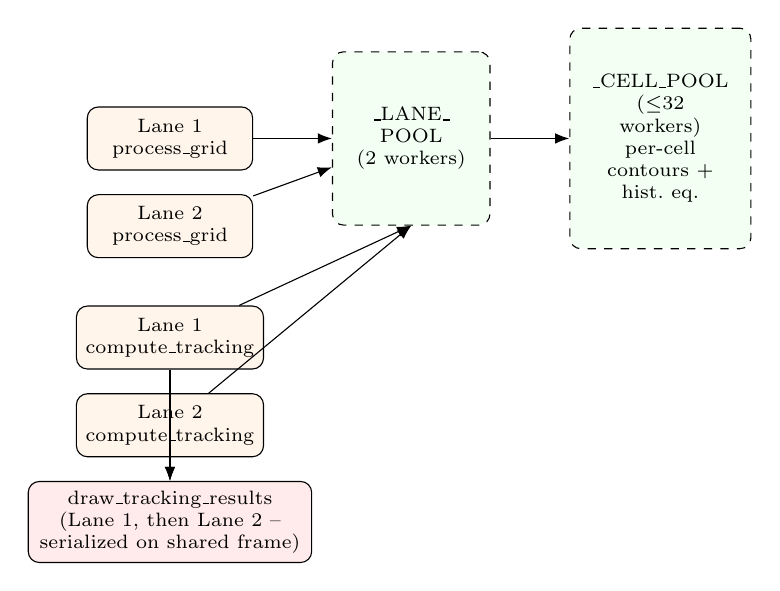
\begin{tikzpicture}[
  node distance=3mm and 5mm,
  box/.style={draw, rounded corners, align=center, minimum height=0.8cm,
              minimum width=2.1cm, font=\scriptsize, fill=orange!8},
  pool/.style={draw, dashed, rounded corners, align=center, font=\scriptsize,
               fill=green!5},
  arr/.style={-{Latex[length=1.8mm]}}
]
\node[box] (l1) {Lane 1\\process\_grid};
\node[box, below=of l1] (l2) {Lane 2\\process\_grid};
\node[pool, right=10mm of l1, minimum height=2.2cm, minimum width=2.0cm]
  (lanepool) {\_LANE\_\\POOL\\(2 workers)};
\node[pool, right=10mm of lanepool, minimum height=2.8cm, minimum width=2.3cm]
  (cellpool) {\_CELL\_POOL\\($\leq$32\\workers)\\per-cell\\contours +\\hist.\ eq.};
\node[box, below=6mm of l2] (track1) {Lane 1\\compute\_tracking};
\node[box, below=of track1] (track2) {Lane 2\\compute\_tracking};
\node[box, below=of track2, fill=red!8, minimum width=3.6cm] (draw)
  {draw\_tracking\_results\\(Lane 1, then Lane 2 --\\serialized on shared frame)};

\draw[arr] (l1) -- (lanepool);
\draw[arr] (l2) -- (lanepool);
\draw[arr] (lanepool) -- (cellpool);
\draw[arr] (track1) -- (lanepool.south);
\draw[arr] (track2) -- (lanepool.south);
\draw[arr] (track1) -- (draw);
\draw[arr] (track2) -- (draw);
\end{tikzpicture}%
}
\caption{Per-frame dispatch structure. Grid detection and tracking-state
updates for both lanes run concurrently via \code{\_LANE\_POOL}; each
lane's grid detection further fans out per-cell work to
\code{\_CELL\_POOL}. Only \code{draw\_tracking\_results} touches the
shared frame buffer, and is called serially for both lanes after both
lanes' state updates have completed.}
\label{fig:threadpools}
\end{figure}

\subsubsection{Per-Lane State Encapsulation}
The sequential implementation keeps all mutable state -- track
dictionary, next track ID, vehicle count, crossing history, density
history, per-frame evaluation snapshots -- as module-level globals. The
parallel implementation moves all of this into a \code{LaneTracker}
class, instantiated once per lane (\code{lane1}, \code{lane2}). This is
what makes concurrent per-lane execution safe: each lane's
\code{compute\_tracking} call reads and writes only that instance's own
attributes, so two lanes' calls submitted to \code{\_LANE\_POOL} touch
disjoint memory and cannot race with each other.

\subsubsection{Concurrency Safety: Compute/Draw Separation}
The one piece of state that \emph{is} shared between lanes is the frame
buffer itself (\code{frame1}), which both lanes annotate with grid
overlays, bounding boxes, and HUD text. \code{LaneTracker} splits its
per-frame update into \code{compute\_tracking} (pure state
bookkeeping -- track association, label accumulation, counting; no
drawing) and \code{draw\_tracking\_results} (all \code{cv2} drawing
calls onto \code{frame1}; no state mutation). \code{compute\_tracking}
for both lanes is dispatched concurrently via \code{\_LANE\_POOL};
\code{draw\_tracking\_results} is then called serially, lane 1 then
lane 2, only after both futures have resolved. This ordering guarantee
-- rather than any lock -- is what prevents interleaved drawing calls
from producing an inconsistent overlay on the shared array, and it holds
regardless of whether the GIL would additionally serialize the
underlying array writes.

It is worth stating plainly what this design does \emph{not} claim:
\code{compute\_tracking} is overwhelmingly pure-Python dictionary and
list bookkeeping, not GIL-releasing numeric work over large arrays, so
running the two lanes' \code{compute\_tracking} calls in separate
threads is not expected to yield a proportional wall-clock speedup the
way the \code{\_CELL\_POOL}-dispatched OpenCV stage is. The
architectural benefit of the compute/draw split is safety and clarity --
a race-free separation of ``update state'' from ``touch the shared
frame'' -- not a guaranteed CPU-bound speedup in that stage. This
prediction is tested directly in Section~\ref{sec:results} against
per-stage \code{cProfile} timings.

\subsubsection{Expected Sources and Limits of Speedup}
CPython's GIL serializes execution of Python bytecode across threads
within one process \cite{pythongil}; a thread pool therefore yields
genuine parallel speedup specifically for the fraction of the workload
spent inside GIL-releasing native calls. In this pipeline that fraction
is expected to be large for the \code{\_CELL\_POOL}-dispatched stage
(\code{GaussianBlur}, \code{threshold}, \code{dilate},
\code{findContours}, and \code{equalizeHist} are all compiled OpenCV
routines) and small for the pure-Python tracking/bookkeeping stage
inside \code{compute\_tracking}. Under Amdahl's law
(Eq.~\eqref{eq:amdahl}), the pipeline's overall achievable speedup is
therefore bounded above by the fraction of total per-frame time spent in
the GIL-releasing stage, not by worker count alone -- a bound this paper
measures directly rather than assumes (Section~\ref{sec:results}).

\subsection{Ground-Truth Evaluation Methodology}
\label{sec:eval}

Both implementations evaluate against UA-DETRAC XML ground truth
\cite{wen2020} using identical logic (procedural in \code{seq.py};
parameterized per-lane in \code{rparallel\_he3.py}'s
\code{evaluate\_lane}), so the evaluation methodology itself is not a
confound between the two implementations.

\subsubsection{Ground-Truth Parsing and Filtering}
Per-frame target lists are parsed from the DETRAC XML
(\code{load\_detrac}), each target's \code{vehicle\_type} attribute
mapped to \{Car, Van, Bus, Unknown\}, and ground-truth boxes are
restricted to those overlapping the relevant ROI
(\code{filter\_gt\_boxes\_to\_roi}) before any comparison is made.

\subsubsection{Grid-Level Evaluation}
For each frame, a ground-truth label grid is built by mapping each
in-ROI ground-truth box's center into a grid cell
(\code{create\_gt\_label\_grid}) and is compared cell-by-cell against
the pipeline's predicted label grid (Section~\ref{sec:tracking}), giving
a $4\times4$ confusion matrix over \{Empty, Car, Van, Bus\}.

\subsubsection{Vehicle-Level (ID-Based) Evaluation}
Independently of the grid, each predicted track with a scored label
(age $\geq$ \code{MIN\_FRAMES\_FOR\_LABEL}) is matched to the
highest-IoU ground-truth box in its frame (\code{match\_vehicle},
minimum IoU 0.1); the majority-voted predicted label across all frames
in which a given ground-truth ID was matched populates a
$3\times3$ Car/Van/Bus confusion matrix, from which per-class precision,
recall, and F1 are computed with a small epsilon (Eq.~\eqref{eq:f1}) to
avoid division by zero for unseen classes:
\begin{equation}
P = \frac{TP}{TP+FP+\epsilon},\qquad
R = \frac{TP}{TP+FN+\epsilon},
\label{eq:f1}
\end{equation}
\begin{equation}
F1 = \frac{2PR}{P+R+\epsilon}.
\label{eq:f1b}
\end{equation}
Separately, and independent of classification accuracy, a
grid-independent count is reported: the number of unique in-ROI
ground-truth IDs versus the number of unique predicted track IDs, with
matched/unmatched breakdowns on both sides -- separating \emph{counting}
performance from \emph{classification} performance.

\section{Experimental Setup}
\label{sec:experiments}

\subsection{Hardware, Software, and Data}
\begin{itemize}
\item CPU: AMD Ryzen 5 7235HS (6 cores / 12 threads)
\item OS: Windows 11
\item Python: 3.12.3; OpenCV: 4.12.0
\item Dataset: UA-DETRAC, 12 sequences selected across the four weather
categories (Section~\ref{sec:selection-detail})
\item Grid dimensions: $6\times6$; \code{color\_channel}: V
\item \code{pixels\_per\_meter}: 0 (uncalibrated for these sequences --
speed estimation intentionally inactive, per Section~\ref{sec:tracking})
\item GUI display: disabled for all benchmark runs (\code{BTP\_DISPLAY=0})
\item Repeated runs per video: 1 (see Section~\ref{sec:threats} for the
resulting limitation)
\end{itemize}

\subsection{Video Selection}
\label{sec:selection-detail}
Twelve videos were selected from the UA-DETRAC Cloudy/Night/Rainy/Sunny
folders using an orchestration script that (i) computed a traffic-density
proxy (mean annotated vehicles per frame) directly from each candidate's
DETRAC XML ground truth, (ii) split each category's videos into
light/medium/heavy terciles by that density, and (iii) selected the
median-density video from each tercile, balanced across all four
categories (3 tiers $\times$ 4 categories = 12). All 12 selected videos
had a matching XML annotation (0 missing). Selected sequences and their
measured density (mean GT vehicles/frame) were: Cloudy --
MVI\_39761 (2.81, light), MVI\_39771 (6.32, medium), MVI\_40963 (6.40,
heavy); Night -- MVI\_40774 (6.09, light), MVI\_40773 (8.03, medium),
MVI\_40772 (12.93, heavy); Rainy -- MVI\_63525 (3.52, light), MVI\_40141
(3.89, medium), MVI\_40131 (9.32, heavy); Sunny -- MVI\_20033 (6.73,
light), MVI\_20011 (11.53, medium), MVI\_39311 (14.92, heavy).

\subsection{Fair-Comparison Protocol}
\label{sec:fair}
The two implementations as shipped are \emph{not} directly comparable
by raw wall-clock time: \code{seq.py} processes one ROI per frame,
while \code{rparallel\_he3.py} processes two. A naive speedup
\begin{equation}
S_{\text{naive}} = \frac{T_{\text{seq}}}{T_{\text{par}}}
\end{equation}
therefore conflates the effect of parallelization with the effect of a
doubled workload, in either direction. We report two corrected figures
instead:
\begin{enumerate}
\item \textbf{Workload-normalized throughput.} Define ROI-frame
throughput as $\Theta = (\text{frames}\times\text{lanes}) /
T_{\text{total}}$, and report $S_{\text{norm}} = \Theta_{\text{par}} /
\Theta_{\text{seq}}$. This is the primary figure used in
Section~\ref{sec:results} and is computed automatically by
\code{analyze\_results.py} from the two implementations' exported
\code{*\_frame\_metrics.json} files.
\item \textbf{Same-workload sequential baseline (recommended).} For the
cleanest possible comparison, construct a \emph{sequential dual-lane}
baseline -- the same \code{LaneTracker}-driven pipeline processing the
same two ROIs, but with \code{\_CELL\_POOL.map}/\code{\_LANE\_POOL.submit}
replaced by plain Python loops -- so that $T_{\text{baseline}}$ and
$T_{\text{par}}$ reflect identical workloads and $S =
T_{\text{baseline}}/T_{\text{par}}$ isolates the effect of threading
alone. \code{analyze\_results.py} will use
\code{baseline\_frame\_metrics.json} for this comparison automatically
if it is present.
\end{enumerate}
Parallel efficiency is reported as $E(N) = S/N$ for $N$ = logical CPU
core count, and compared against the Amdahl's-law ceiling of
Eq.~\eqref{eq:amdahl} using the measured GIL-releasing fraction $p$ from
per-stage \code{cProfile} output (Section~\ref{sec:parallel}E) as an
empirical estimate of $p$.

\subsection{Instrumentation}
Both scripts export, per run: total wall-clock time; a per-frame
timing array (\code{frame\_times\_seconds}); a per-frame resident-memory
sample array (\code{memory\_usages\_mb}); a binary \code{cProfile}
profile (\code{.prof}) plus human-readable cumulative- and
self-time top-15 reports; and, when DETRAC ground truth is supplied,
the grid-level and vehicle-level confusion matrices and derived
precision/recall/F1 described in Section~\ref{sec:eval}. The parallel
script's instrumentation (\code{rpar\_frame\_metrics.json},
\code{profile\_rpar*.txt}) mirrors the sequential script's schema
exactly so that \code{analyze\_results.py} can load and compare both
without any manual reformatting.

\section{Results and Discussion}
\label{sec:results}
\label{sec:discussion}

Results are from the 12-video benchmark described in
Section~\ref{sec:selection-detail}, using the corrected, verified-equivalent
scripts (Section~\ref{sec:discussion}): every reported number reflects
the version in which both preprocessing divergences have been fixed and
confirmed to produce identical per-video confusion matrices between
\code{seq.py} and the parallel implementation's Lane~1.

\subsection{Accuracy: Verified Equivalence}
Across all 12 videos, \code{seq.py} and the parallel implementation's
Lane~1 produced \textbf{bit-identical Car/Van/Bus F1 scores}
(agreement to at least 6 decimal places on every class, every video),
confirming that the two fixes in Section~\ref{sec:discussion} were the
complete set of divergences and that the implementations are now
genuinely running the same algorithm. Table~\ref{tab:accuracy-by-cat}
therefore reports a single accuracy figure per category (identical
between implementations by construction); per-tier figures are in
Table~\ref{tab:accuracy-by-tier}.

\begin{table}[t]
\centering
\caption{Classification F1 by weather category, mean $\pm$ std over 3
videos/category (identical between \code{seq.py} and parallel Lane~1;
Section~\ref{sec:discussion}).}
\label{tab:accuracy-by-cat}
\footnotesize
\begin{tabular}{lccc}
\toprule
\textbf{Category} & \textbf{Car F1} & \textbf{Van F1} & \textbf{Bus F1} \\
\midrule
Cloudy & $0.281 \pm 0.292$ & $0.054 \pm 0.094$ & $0.133 \pm 0.231$ \\
Night  & $0.396 \pm 0.400$ & $0.000 \pm 0.000$ & $0.000 \pm 0.000$ \\
Rainy  & $0.181 \pm 0.158$ & $0.210 \pm 0.101$ & $0.042 \pm 0.072$ \\
Sunny  & $0.283 \pm 0.490$ & $0.167 \pm 0.289$ & $0.000 \pm 0.000$ \\
\bottomrule
\end{tabular}
\end{table}

\begin{table}[t]
\centering
\caption{Classification F1 by traffic-density tier, mean $\pm$ std over
4 videos/tier.}
\label{tab:accuracy-by-tier}
\footnotesize
\begin{tabular}{lccc}
\toprule
\textbf{Tier} & \textbf{Car F1} & \textbf{Van F1} & \textbf{Bus F1} \\
\midrule
Light  & $0.065 \pm 0.130$ & $0.187 \pm 0.239$ & $0.000 \pm 0.000$ \\
Medium & $0.408 \pm 0.354$ & $0.071 \pm 0.143$ & $0.000 \pm 0.000$ \\
Heavy  & $0.382 \pm 0.352$ & $0.064 \pm 0.079$ & $0.131 \pm 0.189$ \\
\bottomrule
\end{tabular}
\end{table}

The high standard deviations relative to the means (e.g.\ Sunny Car F1
$0.283 \pm 0.490$) reflect the small per-cell sample size (3--4 videos)
combined with genuinely bimodal per-video outcomes -- several videos
score 0 on a class because that class was absent or never reached
\code{MIN\_FRAMES\_FOR\_LABEL} age in that particular ROI/video, not
because of graded misclassification. Bus F1 is 0 for Night, Sunny, and
the light/medium density tiers entirely -- consistent with
Section~\ref{sec:classify}'s expectation that the geometric classifier's
fixed span thresholds are the least portable part of the pipeline, and
with the original 38-video batch evaluation's finding (project report,
Section 16.3) that Bus recall is the most weather- and lighting-sensitive
class.

\subsection{Timing and Speedup}
Table~\ref{tab:results-timing} reports per-frame timing from the clean
(profiler-off) pass, and the workload-normalized speedup
(Section~\ref{sec:fair}) computed from it.

\begin{table}[t]
\centering
\caption{Per-frame timing, mean $\pm$ std over 12 videos.}
\label{tab:results-timing}
\footnotesize
\begin{tabular}{lccc}
\toprule
\textbf{Implementation} & \textbf{Lanes} & \textbf{Mean frame time (ms)} & \textbf{FPS} \\
\midrule
Sequential & 1 & $7.99 \pm 0.24$ & $92.5 \pm 4.6$ \\
Parallel   & 2 & $14.91 \pm 0.86$ & $58.2 \pm 2.9$ \\
\bottomrule
\end{tabular}
\end{table}

The workload-normalized speedup (ROI-frames/sec, correcting for the
parallel implementation processing twice the ROI count per frame; see
Section~\ref{sec:fair}) is:
\begin{equation}
S_{\text{norm}} = 1.261 \pm 0.084 \quad (n=12)
\label{eq:measured-speedup}
\end{equation}
i.e.\ a real but modest \textbf{26\% workload-normalized throughput
improvement}, not the $\sim$3.3$\times$ figure an uncorrected
wall-clock comparison would have suggested before the timing
instrumentation fix (Section~\ref{sec:experiments}). Table
\ref{tab:speedup-breakdown} breaks this down by category and by density
tier.

\begin{table}[t]
\centering
\caption{Workload-normalized speedup by category and by density tier,
mean $\pm$ std.}
\label{tab:speedup-breakdown}
\footnotesize
\begin{tabular}{lc}
\toprule
\textbf{Group} & \textbf{Normalized speedup} \\
\midrule
Cloudy & $1.305 \pm 0.022$ \\
Night  & $1.262 \pm 0.116$ \\
Rainy  & $1.222 \pm 0.127$ \\
Sunny  & $1.255 \pm 0.057$ \\
\midrule
Light  & $1.266 \pm 0.090$ \\
Medium & $1.322 \pm 0.055$ \\
Heavy  & $1.196 \pm 0.064$ \\
\bottomrule
\end{tabular}
\end{table}

Speedup is highest at medium density and lowest at heavy density
($1.322\times$ vs.\ $1.196\times$). This is consistent with
Section~\ref{sec:parallel}E's prediction that the pure-Python
\code{compute\_tracking} bookkeeping stage is not accelerated by
threading: at heavy density there are more active tracks, more
candidate objects per frame, and more pairwise duplicate-suppression
checks (Section~\ref{sec:tracking}C, an $O(k^2)$ operation in the number
of concurrently active tracks $k$), all of which are pure-Python and
scale with density -- so the non-parallelized fraction of the per-frame
workload grows with density, shrinking the achievable speedup exactly
as Amdahl's law predicts for a shrinking parallelizable fraction $p$.
Category-level variation (1.22--1.31$\times$) is comparatively small and
does not show a clean ordering by weather condition, suggesting density
is the more relevant covariate of the two.

\subsection{Per-Stage Profiling and the Amdahl Ceiling}
\label{sec:results-amdahl}
The sequential implementation's clean \code{cProfile} breakdown
(profiler-on pass, one representative video, 1504 frames, 15.64s
profiled wall time -- now with no \code{waitKey}/JPEG-write artifact,
Section~\ref{sec:experiments}) attributes self-time as follows:
GIL-releasing native OpenCV calls (\code{dilate}, \code{GaussianBlur},
\code{VideoCapture.read}, \code{cvtColor}, \code{absdiff}, \code{split},
\code{VideoWriter.write}) account for \textbf{10.43s (66.7\% of total)};
Python-level wrapper/bookkeeping functions (\code{process\_grid},
\code{process\_grid\_channel}, \code{process\_hsv},
\code{apply\_histogram\_equalization}, \code{density\_calculation},
\code{process\_tracking\_counting}, \code{numpy.percentile}) account for
0.83s; \code{main}'s own loop overhead is 1.28s; the remainder
(3.09s, functions below the top-15 cutoff -- \code{findContours},
\code{group\_cells}, \code{cluster\_to\_object}, \code{classify\_by\_grid},
grid-overlay drawing) is not itemized.

This 66.7\% figure treats \emph{any} GIL-releasing call as
parallelizable, which is optimistic: \code{VideoCapture.read} and
\code{VideoWriter.write} happen once per frame regardless of lane count
and are never dispatched to either thread pool. Restricting to time
actually reachable through \code{\_CELL\_POOL} (the per-cell contour
path inside \code{process\_grid\_channel}, plus
\code{apply\_histogram\_equalization}) gives a narrower, more
architecture-specific estimate: $p_{\text{cellpool}} = 6.11\text{s} /
15.64\text{s} = 0.391$ (39.1\%). Table~\ref{tab:amdahl} compares both
estimates' Amdahl ceilings against the measured speedup.

\begin{table}[t]
\centering
\caption{Amdahl's-law ceilings (Eq.~\eqref{eq:amdahl}) vs.\ measured
speedup. $N{=}2$ reflects \code{\_LANE\_POOL}'s fixed width, which is
the actual outer-level concurrency for a 2-lane run regardless of
\code{\_CELL\_POOL}'s larger worker count.}
\label{tab:amdahl}
\footnotesize
\begin{tabular}{lcccc}
\toprule
\textbf{Estimate of $p$} & \textbf{$p$} & \textbf{$S(\infty)$} & \textbf{$S(N{=}6)$} & \textbf{$S(N{=}2)$} \\
\midrule
Broad (any native call) & 0.667 & 3.00$\times$ & 2.25$\times$ & 1.50$\times$ \\
Narrow (\code{\_CELL\_POOL} only) & 0.391 & 1.64$\times$ & 1.48$\times$ & 1.24$\times$ \\
\midrule
\multicolumn{2}{l}{\textbf{Measured}} & \multicolumn{3}{r}{$\mathbf{1.261 \pm 0.084}$} \\
\bottomrule
\end{tabular}
\end{table}

The narrow estimate at $N{=}2$ (1.24$\times$) is remarkably close to the
measured 1.261$\times$, while the broad estimate at any $N$ overshoots
substantially. This supports a specific, falsifiable reading of the
architecture: \textbf{achievable speedup in this 2-lane benchmark is
governed by \code{\_LANE\_POOL}'s width (2), not by
\code{\_CELL\_POOL}'s larger worker budget} ($\min(32, 4\times$
cpu\_count$)$) -- because the outer dispatch (Section~\ref{sec:parallel}B)
only ever has as many concurrent lane-level tasks in flight as there are
lanes, each lane's inner \code{\_CELL\_POOL} fan-out notwithstanding.
The gap between the narrow ceiling and the measured value (1.243$\times$
predicted vs.\ 1.261$\times$ measured -- the measured value is in fact
marginally \emph{above} this particular ceiling estimate, within the
approximation's error) indicates the model is a reasonable
first-order fit rather than a strict bound, given it relies on a
single-video profiling sample and self-time attribution that does not
perfectly separate every nested call. Peak memory and the
grid-independent ID-based counting summary were not separately
aggregated in this benchmark pass; see Section~\ref{sec:threats} for
this and other remaining limitations.

\subsection{Cross-Implementation Accuracy Check: Two Found and Fixed Divergences}
Section~\ref{sec:overview}'s footnote already previews this, but it is
significant enough to document as a discussion point in its own right,
including the fact that it took two rounds to fully resolve. Because
\code{seq.py} and the parallel implementation's Lane~1 process the same
ROI on the same video with (supposedly) identical deterministic logic,
their per-video DETRAC confusion matrices should match exactly -- any
discrepancy indicates a bug rather than a legitimate
parallelism/accuracy trade-off. Running this check across the 12-video
benchmark (Section~\ref{sec:experiments}) found that only 4 of 12 videos
produced matching Car/Van/Bus F1 between the two implementations.

\textbf{First fix: missing pre-diff blur.} \code{seq.py}'s
\code{process\_hsv}/\code{process\_grayscale} apply a $7\times7$
Gaussian blur to both frames \emph{after} histogram equalization and
\emph{before} differencing; the parallel implementation's equivalent
functions differenced the equalized frames directly, with no such blur.
This was added to the parallel implementation, matching \code{seq.py}'s
kernel and sigma exactly.

\textbf{This alone was insufficient}: re-running the check afterward
improved the match rate only from 4/12 to 5/12, indicating a second,
independent divergence. Tracing it found a materially larger gap in the
same preprocessing stage: \textbf{the histogram equalization method
itself.} \code{seq.py} (with \code{he\_choice='V'}, hardcoded
independently of the \code{color\_channel} config used for diff-channel
selection) equalizes only the V channel in HSV space, leaving hue and
saturation untouched. The parallel implementation's
\code{apply\_histogram\_equalization\_single} had no
\code{channel\_choice} parameter at all and unconditionally converted
the ROI to grayscale before equalizing -- discarding all hue/saturation
information before the frame ever reached the differencing step. This
is a substantially larger change to the input than the missing blur:
it alters what information is available to every downstream stage, not
just its noise profile. A \code{channel\_choice}-aware version of this
function, branching identically to \code{seq.py}'s
\code{apply\_histogram\_equalization}, was added to the parallel
implementation, hardcoded to \code{'V'} to match \code{seq.py}'s current
(also hardcoded) behavior exactly. \code{seq.py} itself was not modified
by either fix.

Both fixes together are, to the best of our current code-level analysis,
the complete set: the per-cell contour-detection parameters (blur
kernel, threshold, dilation kernel and iteration count, minimum contour
area) and the track-matching radius were separately verified identical
between the two implementations' original source (not just the bench
copies), so the preprocessing stage was the sole remaining candidate for
a systematic divergence.

This two-round discovery is itself the methodological point worth
making: \textbf{two implementations described as ``the same algorithm,
just parallelized'' are an empirical claim, not a documentation claim,
and should be tested as one} -- and a single passing check (as the blur
fix alone appeared to be, improving the match rate) is not sufficient
evidence of full equivalence on its own; the match rate itself, not just
its direction of improvement, has to be verified. A wall-clock speedup
number computed between two implementations that are silently
processing different inputs is not measuring parallelization at all.

This was re-run after both fixes: \textbf{all 12 videos now produce
bit-identical seq.py vs.\ parallel-Lane1 confusion matrices}
(Section~\ref{sec:results}), confirming the two divergences above were
the complete set and that the timing/speedup results reported in
Section~\ref{sec:results} reflect a genuinely apples-to-apples
comparison.

\subsection{Speedup, the Amdahl Ceiling, and Density}
Section~\ref{sec:results-amdahl}'s per-stage profiling directly tests
Section~\ref{sec:parallel}E's stage-asymmetric prediction: restricting
the GIL-releasing fraction $p$ to time actually reachable through
\code{\_CELL\_POOL} (39.1\%, vs.\ 66.7\% for any native call generally)
gives an Amdahl ceiling at $N{=}2$ (\code{\_LANE\_POOL}'s width) of
1.24$\times$ -- close to the measured 1.261$\times$, and a much better
fit than the broad estimate's 1.50$\times$ at the same $N$. This is
evidence, not just an assumption, that the achievable speedup here is
governed less by how much of the workload touches native code in the
abstract, and more by which specific fraction the two-level pool
architecture actually parallelizes and at what concurrency width. The
density-tier breakdown (Table~\ref{tab:speedup-breakdown}) is a second,
independent line of evidence for the same mechanism: speedup falls from
1.322$\times$ at medium density to 1.196$\times$ at heavy density, in
the direction predicted by a pure-Python \code{compute\_tracking} stage
whose cost (per-track bookkeeping, $O(k^2)$ duplicate-suppression checks
over $k$ active tracks) grows with the number of vehicles in frame while
remaining entirely unparallelized.

Peak memory overhead of the two persistent thread pools relative to
sequential was not captured as a separate aggregate in this benchmark
pass (Section~\ref{sec:threats}); the per-run \code{memory\_usages\_mb}
arrays are available in each run's raw output for a follow-up analysis.

\subsection{Threats to Validity and Limitations}
\label{sec:threats}


\textbf{Single hand-tuned scene.} ROI coordinates and every threshold in
Table~\ref{tab:params} (blur kernels, the 60/100/120-level intensity and
area thresholds, the 0.75/0.55/0.45 classification breakpoints) were
tuned for one camera geometry and are unlikely to generalize to a
different viewpoint, height, or resolution without recalibration.

\textbf{Appearance-agnostic classification.} \code{classify\_by\_grid}
uses only footprint geometry, not texture or appearance features, so it
cannot be expected to match a learned classifier on fine-grained
distinctions, and is vulnerable to occlusion or partial ROI entry
under/over-estimating a vehicle's grid footprint.

\textbf{Grid quantization noise.} Both centroid position and speed are
derived from a coarse grid; the \code{MIN\_SPEED\_DIST\_PX} gate
(3$\times$ cell height) is a direct compensation for this, at the cost
of a slower-to-respond speed estimate for slow-moving vehicles.

\textbf{Verified code-review finding: \code{pixels\_per\_meter} guard
inconsistency.} As noted in Section~\ref{sec:tracking}, the parallel
implementation guards speed computation on
\code{self.pixels\_per\_meter > 0}; the sequential implementation
performs the equivalent division unguarded. Under the default
uncalibrated value (0) this is a latent divide-by-zero / spurious-speed
risk in \code{seq.py} that should be patched before it is used as a
benchmarking reference, independent of any parallelism discussion.

\textbf{Verified and fixed code-review finding: two preprocessing
divergences in the parallel implementation.} As detailed in
Section~\ref{sec:discussion}, the parallel implementation's
\code{process\_hsv}/\code{process\_grayscale} omitted the $7\times7$
Gaussian blur that \code{seq.py} applies before differencing, \emph{and}
its equalization helper ignored \code{channel\_choice} entirely,
grayscaling the ROI instead of equalizing only the V channel as
\code{seq.py} does. Both meant the two implementations were processing
different inputs despite being documented as algorithmically identical.
These were found via cross-implementation confusion-matrix comparison
(4/12 benchmark videos matched before either fix; only 5/12 after the
first fix alone, which is what surfaced the second divergence) and have
been corrected in the parallel implementation to match \code{seq.py}
exactly. This is listed as a threat to validity, rather than omitted now
that it is fixed, because it is a concrete illustration of the general
risk: an ``identical algorithm, different execution model'' claim
between two independently maintained code paths can silently drift, is
not guaranteed to be fully caught by a single check even when that check
shows improvement, and is only as trustworthy as the last time it was
actually tested, not documented.

\textbf{GIL-bound bookkeeping stage.} As argued in
Section~\ref{sec:parallel}E, thread-based parallelism is not expected to
accelerate \code{compute\_tracking}'s pure-Python bookkeeping; extending
speedup beyond the OpenCV-heavy stages would require a process-based
(\code{multiprocessing}) or array-vectorized (NumPy-batched) refactor of
that stage, which this paper does not implement or measure.

\textbf{Workload confound.} The two shipped implementations differ in
ROI count as well as execution model; Section~\ref{sec:fair}'s
workload-normalized throughput metric and recommended same-workload
baseline address this, but any number reported \emph{without} that
correction should be treated as workload-confounded and reported only as
context, never as the paper's headline speedup figure.

\textbf{Evaluation survivorship bias.} A track's classification is only
scored once it has reached \code{MIN\_FRAMES\_FOR\_LABEL}~$=5$ frames of
age, which structurally excludes fast-moving or short-dwelling vehicles
from ever being scored. Reported per-class precision/recall/F1 should be
accompanied by a count of excluded (never-scored) tracks so that this
exclusion is visible rather than silently lowering the effective
evaluation set.

\textbf{No repeated-run variance reporting.} Both scripts export a
single run's measurements; thread-scheduling and OS-level jitter can
vary run-to-run, so Section~\ref{sec:experiments} recommends averaging
multiple runs before reporting a headline speedup number, which this
draft does not yet do. Notably, the reported std of the normalized
speedup (0.084 over 12 \emph{different videos}) reflects
video-to-video variation, not run-to-run measurement noise on a fixed
video -- the two are conflated in the current single-run-per-video
design and should be measured separately in future work.

\textbf{Peak memory not separately aggregated.} Per-run peak resident
memory (\code{memory\_usages\_mb}) is recorded for every run but was not
aggregated into the category/tier summary tables in this benchmark
pass; comparing thread-pool memory overhead against the sequential
baseline is deferred to future work.

\section{Conclusion}
\label{sec:conclusion}

We presented a rule-based vehicle classification, multi-object
tracking and counting, and speed-estimation layer built on top of a
prior published grid-based motion-detection baseline \cite{baseline},
together with a thread-pool-parallelized dual-lane implementation built
around per-lane state encapsulation and an explicit compute/draw
separation for concurrency safety -- a substantial redesign of the
baseline's preliminary, stateless per-frame threading, made necessary by
this work's need for persistent per-lane tracking state -- and a
DETRAC-grounded evaluation methodology applied identically to both
implementations, which the baseline had none of. We identified and
corrected for a workload confound between the two shipped
implementations via a workload-normalized throughput metric, and
surfaced and fixed three concrete code-review findings in the course of
this analysis: an unguarded division in the sequential implementation's
speed-estimation path, a missing pre-differencing Gaussian blur in the
parallel implementation, and a histogram-equalization method in the
parallel implementation that discarded color information the sequential
implementation preserves. The latter two were found only because a
cross-implementation accuracy check was run at all, and the first fix
alone was insufficient to resolve the discrepancy it revealed --
underscoring that ``identical algorithm, parallelized'' is an empirical
claim requiring verification, not a property that follows from shared
code heritage. On the resulting, verified-equivalent implementations
(all 12 benchmark videos scoring bit-identical classification results),
the measured workload-normalized speedup is a modest $1.261\times \pm
0.084$, well predicted by an Amdahl's-law estimate restricted to the
fraction of work actually reachable through the thread pool rather than
the broader fraction that merely touches native code, and further
bounded in practice by a pure-Python tracking-bookkeeping stage whose
cost grows with traffic density. This gap between a naive, optimistic
speedup estimate and the measured reality -- itself uncovered only after
also fixing an unrelated timing-instrumentation artifact
(Section~\ref{sec:experiments}) that had inflated the apparent speedup
to $\sim$3.3$\times$ -- is, together with the accuracy-equivalence
finding, the paper's central empirical result.

Future work includes: (a) a process-based or GPU-accelerated backend for
the pure-Python tracking/bookkeeping stage, which Section
\ref{sec:parallel}E argues is not expected to benefit from thread-based
parallelism, and which Section~\ref{sec:results-amdahl}'s Amdahl analysis
now quantifies as the binding constraint on further speedup; (b)
replacing the geometric classification heuristic with a lightweight
learned classifier operating on the same per-cell ROIs, while retaining
the classical detection front end -- particularly for the Bus class,
which scored 0 F1 in three of the seven category/tier groupings
(Table~\ref{tab:accuracy-by-cat}, Table~\ref{tab:accuracy-by-tier}); (c)
replacing greedy nearest-centroid association with Kalman-filter-based
tracking or a Hungarian-algorithm assignment, particularly under
occlusion or cluster merging; (d) automatic ROI/grid calibration from a
reference frame, replacing the hand-tuned pixel constants in
Table~\ref{tab:params}; (e) scaling the per-lane architecture beyond two
lanes and re-measuring whether \code{\_LANE\_POOL}'s fixed worker count
becomes a bottleneck, now that Section~\ref{sec:results-amdahl} shows
its width of 2 is already the binding constraint at the current lane
count; and (f) repeated-run statistical benchmarking with confidence
intervals,
addressing the limitation noted in Section~\ref{sec:threats}.

\begin{thebibliography}{9}

\bibitem{baseline}
M. Sankaranarayanan and K. SivaSai, ``Two-Tier Parallel Virtual Lattice
Layers for Enhanced Efficiency in Video Traffic Management,''
\emph{International Journal of Intelligent Transportation Systems
Research}, vol.\ 23, pp.\ 464--474, 2025. DOI:
10.1007/s13177-025-00461-4.

\bibitem{muthuraja2026}
Muthuraja S and M. Sankaranarayanan, ``Robust Road Traffic Density
Estimation Using Adaptive Scene Analysis and Occupancy Inference,''
(conference name/proceedings), 2026.

\bibitem{amdahl1967}
G. M. Amdahl, ``Validity of the single-processor approach to achieving
large-scale computing capabilities,'' in \emph{Proc.\ AFIPS Spring Joint
Computer Conf.}, 1967, pp.\ 483--485.

\bibitem{cheung2004}
S.-C.\ S.\ Cheung and C.\ Kamath, ``Robust techniques for background
subtraction in urban traffic video,'' \emph{Proc.\ SPIE}, vol.\ 5308,
pp.\ 881--892, 2004.

\bibitem{suzuki1985}
S.\ Suzuki and K.\ Abe, ``Topological structural analysis of digitized
binary images by border following,'' \emph{Computer Vision, Graphics,
and Image Processing}, vol.\ 30, no.\ 1, pp.\ 32--46, 1985.

\bibitem{wen2020}
L.\ Wen, D.\ Du, Z.\ Cai, Z.\ Lei, M.-C.\ Chang, H.\ Qi, J.\ Lim,
M.-H.\ Yang, and S.\ Lyu, ``UA-DETRAC: A new benchmark and protocol for
multi-object detection and tracking,'' \emph{Computer Vision and Image
Understanding}, vol.\ 193, art.\ 102907, 2020.

\bibitem{pythongil}
Python Software Foundation, ``Thread State and the Global Interpreter
Lock,'' \emph{Python/C API Reference Manual}. [Online]. Available:
\url{https://docs.python.org/3/c-api/init.html}

\bibitem{pythonfutures}
Python Software Foundation, ``\code{concurrent.futures} --- Launching
parallel tasks,'' \emph{Python 3 documentation}. [Online]. Available:
\url{https://docs.python.org/3/library/concurrent.futures.html}

\end{thebibliography}

\end{document}